\usetikzlibrary{arrows.meta,calc}
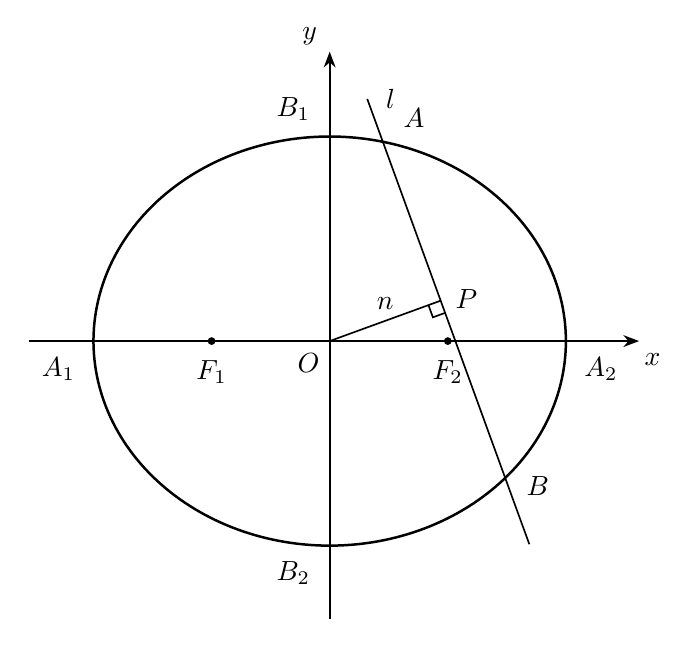
\begin{tikzpicture}[x=1.5cm,y=1.5cm,line width=.6pt,font=\normalsize,inner sep=0pt,>=Stealth]
\coordinate (O) at (0,0);
\coordinate (A1) at (-2.000000,0);
\coordinate (A2) at (2.000000,0);
\coordinate (B1) at (0,1.732051);
\coordinate (B2) at (0,-1.732051);
\coordinate (F1) at (-1.000000,0);
\coordinate (F2) at (1.000000,0);
\coordinate (P) at (0.939693,0.342020);
\coordinate (A) at (0.449922,1.687655);
\coordinate (B) at (1.486081,-1.159169);
\coordinate (lup) at (0.318039,2.050000);
\coordinate (ldn) at (1.690207,-1.720000);
\coordinate (RA1) at (0.836326,0.304398);
\coordinate (RA2) at (0.977315,0.238654);
\coordinate (RA3) at (0.873949,0.201032);
\draw[->] (-2.55,0)--(2.62,0);
\draw[->] (0,-2.35)--(0,2.45);
\draw[line width=.9pt] plot[domain=0:360,samples=240] ({2*cos(\x)},{sqrt(3)*sin(\x)});
\draw (O)--(P);
\draw (lup)--(ldn);
\draw (RA1)--(RA3)--(RA2);
\fill (F1) circle[radius=1.4pt];
\fill (F2) circle[radius=1.4pt];
\node[anchor=north east] at (-0.08,-0.10) {$O$};
\node[anchor=east] at (-2.15,-0.24) {$A_1$};
\node[anchor=west] at (2.15,-0.24) {$A_2$};
\node[anchor=south east] at (-0.16,1.86) {$B_1$};
\node[anchor=north east] at (-0.16,-1.86) {$B_2$};
\node[anchor=north] at (-1.00,-0.16) {$F_1$};
\node[anchor=north] at (1.00,-0.16) {$F_2$};
\node[anchor=west] at (1.06,0.36) {$P$};
\node[anchor=south west] at (0.62,1.80) {$A$};
\node[anchor=north west] at (1.66,-1.14) {$B$};
\node[anchor=south west] at (0.47,1.96) {$l$};
\node[anchor=south] at (0.47,0.26) {$n$};
\node[anchor=north west] at (2.66,-0.10) {$x$};
\node[anchor=south east] at (-0.10,2.50) {$y$};
\end{tikzpicture}
